%iffalse
\let\negmedspace\undefined
\let\negthickspace\undefined
\documentclass[journal,12pt,onecolumn]{IEEEtran}
\usepackage{cite}
\usepackage{amsmath,amssymb,amsfonts,amsthm}
\usepackage{algorithmic}
\usepackage{graphicx}
\usepackage{textcomp}
\usepackage{xcolor}
\usepackage{txfonts}
\usepackage{listings}
\usepackage{enumitem}
\usepackage{mathtools}
\usepackage{gensymb}
\usepackage{comment}
\usepackage{multicol}
\usepackage[breaklinks=true]{hyperref}
\usepackage{tkz-euclide} 
\usepackage{listings}
\usepackage{gvv}                                        
%\def\inputGnumericTable{}                                 
\usepackage[latin1]{inputenc}                                
\usepackage{color}                                            
\usepackage{array}                                            
\usepackage{longtable}                                       
\usepackage{calc}                                             
\usepackage{multirow}                                         
\usepackage{hhline}                                           
\usepackage{ifthen}                                           
\usepackage{lscape}
\usepackage{tabularx}
\usepackage{array}
\usepackage{float}
\usepackage{circuitikz}

\newtheorem{theorem}{Theorem}[section]
\newtheorem{problem}{Problem}
\newtheorem{proposition}{Proposition}[section]
\newtheorem{lemma}{Lemma}[section]
\newtheorem{corollary}[theorem]{Corollary}
\newtheorem{example}{Example}[section]
\newtheorem{definition}[problem]{Definition}
\newcommand{\BEQA}{\begin{eqnarray}}
\newcommand{\EEQA}{\end{eqnarray}}
\renewcommand{\define}{\stackrel{\triangle}{=}}
\theoremstyle{remark}
\newtheorem{remark}{Remark}

% Marks the beginning of the document
\begin{document}
\bibliographystyle{IEEEtran}
\vspace{3cm}

\title{ae-$2013$-$40$ to $52$}
\author{AI24BTECH11020 - Rishika}
\maketitle
\bigskip
\renewcommand{\thefigure}{\theenumi}
\renewcommand{\thetable}{\theenumi}
\begin{enumerate}[start=40]
\item A horizontal rectangular plate $ABCD$ is hinged at points $A, B$ and $C$. $AC$ and $BD$ are diagonals of the plate. Downward force $P$ is applied at $D$. The upward reactions $R_A,R_B$ and $R_C$ at points $A, B$ and $C$, respectively, are
	\begin{enumerate}
		\item indeterminate
		\item $P,-P,P$
		\item $0,P,0$
		\item $\frac{P}{3},\frac{P}{3},\frac{P}{3}$
	\end{enumerate}
\item In the steel structure(Young's modulus = $200 GPa$) shown in the figure, all members have a circular cross-section of radius $10 mm$. Column BD is pinned at $B$ and $D$. The support at $A$ is hinged. The minimum value of load at $P$ at which the column $BD$ may buckle in Newtons is approximately \underline{\hspace{2cm}} \\
	\begin{center}\begin{tikzpicture}
		 \draw (-4,0.2)rectangle(4,-0.2);
        \draw (0,0) circle (2mm);\draw (-3.8,0) circle (2mm);
    \draw (-3.9,-0.2) -- (-4.1,-0.7) -- (-3.5,-0.7)--(-3.7,-0.2);
    \draw(-0.2,0)--(-0.2,-4)--(0.2,-4)--(0.2,0);
    \draw (0,-3.8) circle (2mm);
    \draw(-0.1,-4)--(-0.3,-4.5)--(0.3,-4.5)--(0.1,-4);
    \draw[<->] (-4,0.4)--(0,0.4);\node at (-3.8,0.7) {$A$};
    \draw[<->] (4,0.4)--(0,0.4);\node at (3.8,0.7) {$C$};
    \node at (0,0.7) {$B$};
    \node at (-2,0.7) {$1m$};\node at (2,0.7) {$1m$};
    \draw[->] (4,-0.2)--(4,-1);\node at (4.2,-1) {$P$};
    \draw[<->] (0.4,-0.2)--(0.4,-4);\node at (0.8,-2) {$2m$};
    \node at (0.8,-3.8) {$D$};
	\end{tikzpicture}\end{center}
\item The thin rectangular plate has dimensions $L\times b\times t.$ It develops a stress field corresponding to an applied bending moment $M$ as shown in the figure. A valid Airy's stress function is\\\begin{center}\begin{tikzpicture}
    \draw (-4,1)rectangle (4,-1);
    \draw[->] (-4.2,-1) .. controls (-5,0) .. (-4.2,1);
    \draw[->] (4.2,-1) .. controls (5,0) .. (4.2,1); 
    \draw[<->] (-2.5,1)--(-2.5,-1);
    \draw[<-] (-4,-1.3) -- (-0.5,-1.3);
    \node at(0,-1.3){$L$};
    \draw[->] (0.5,-1.3)--(4,-1.3);
    \draw[->] (0,0)--(0,1.5);\draw[->](0,0)--(5,0);
    \node at (-2,0) {$b$};
        \node at (-5,0.5) {$M$};
        \node at (5,0.5) {$M$};
        \node at (-0.3,1.4) {$y$};
        \node at (5.3,-0.2) {$x$};
\end{tikzpicture}
\end{center}
\begin{enumerate}
	\item $\frac{2M}{tb^3}x^3$
	\item $\frac{2M}{tb^3}y^3$
	\item $\frac{2M}{tb^3}\brak{x^3+y^3}$
	\item $\frac{2M}{tb^3}y^4$
\end{enumerate}
\item A cantilever beam of negligible mass is $0.6 m$ long. It has a rectangular cross-section of width $8 mm$ and thickness $6 mm$ and carries a tip of mass $1.4 kg$. If the natural frequency of this system is $10 rad/sec$, Young's modulus of the material of the beam in $GPa$ is \underline{\hspace{2cm}} \\
\item A simply supported beam with overhang is loaded by uniformly distributed load of intensity $q$ as shown in the figure. The bending moment at the mid-point of $AB$ is
	\begin{center}
    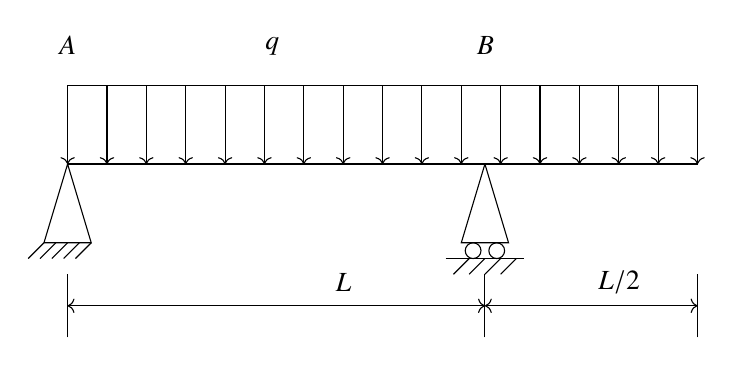
\begin{tikzpicture}
\draw[<->](0,-1)--(0,0)--(8,0)--(8,-1);
\draw[->] (0.5,0)--(0.5,-1);\draw[->] (1,0)--(1,-1);
\draw[->] (1.5,0)--(1.5,-1);\draw[->] (2,0)--(2,-1);
\draw[->] (2.5,0)--(2.5,-1);\draw[->] (3,0)--(3,-1);
\draw[->] (3.5,0)--(3.5,-1);\draw[->] (4,0)--(4,-1);
\draw[->] (4.5,0)--(4.5,-1);\draw[->] (5,0)--(5,-1);
\draw[->] (5.5,0)--(5.5,-1);\draw[->] (6,0)--(6,-1);
\draw[->] (6.5,0)--(6.5,-1);\draw[->] (7,0)--(7,-1);
\draw[->] (7.5,0)--(7.5,-1);
\draw (0,-1)--(8,-1);
\draw (0,-1)--(-0.3,-2)--(0.3,-2)--(0,-1);
\draw(-0.3,-2)--(-0.5,-2.2);
\draw(-0.15,-2)--(-0.35,-2.2);
\draw(0,-2)--(-0.2,-2.2);
\draw(0.15,-2)--(-0.05,-2.2);
\draw(0.3,-2)--(0.1,-2.2);
\draw(5.3,-2.2)--(5.1,-2.4);
\draw(5.5,-2.2)--(5.3,-2.4);
\draw(5.7,-2.2)--(5.5,-2.4);
\draw(5.1,-2.2)--(4.9,-2.4);
\draw (5.3,-1)--(5,-2)--(5.6,-2)--(5.3,-1);
\draw (5.15,-2.1) circle (1mm);
\draw (5.45,-2.1) circle (1mm);
\draw(4.8,-2.2)--(5.8,-2.2);
\draw[<->] (0,-2.8)--(5.3,-2.8);
\draw[<->] (5.3,-2.8)--(8,-2.8);
\draw (0,-3.2)--(0,-2.4);
\draw (5.3,-3.2)--(5.3,-2.4);
\draw (8,-3.2)--(8,-2.4);
\node at(0,0.5){$A$};
\node at(2.6,0.5){$q$};
\node at(5.3,0.5){$B$};
\node at(7,-2.5){$L/2$};
\node at(3.5,-2.5){$L$};
    \end{tikzpicture}
\end{center}
\begin{enumerate}
	\item $\frac{qL^2}{16}$ sagging
	\item $\frac{qL^2}{16}$ hogging
	\item $\frac{3qL^2}{16}$ hogging
	\item $\frac{3qL^2}{16}$ sagging
\end{enumerate}
\item Thrust of liquid oxygen - liquid hydrogen rocket engine is $300 kN$. The O/F ratio used is 5. If the fuel mass flow rate is $12.5 kg/s$, the specific impulse of the rocket motor in $Ns/kg$ is
	\begin{enumerate}
		\item $3800$
		\item $4000$
		\item $4200$
		\item $4400$
	\end{enumerate}
\item In a $50\%$ reaction axial compressor stage, the local blade velocity is $300 m/s$ and the axial component of velocity is $100 m/s$. If the absolute inlet flow angle $\alpha _1=45\degree$, the work per unit mass down on the fluid by the stage in $KJ/kg$ is
	\begin{enumerate}
	\item 30 \item 40 \item 50 \item 60
	\end{enumerate}
\item Consider two rockets $P$ and $Q$ fired vertically up with identical specific impulse and a payload of $2 kg$. Rocket $P$ has $2$ identical stages, and each stage has $200 kg$ of propellant and $20 kg$ of structural weight. Rocket $Q$ has a single stage with $400 kg$ of propellant and $40 kg$ of structural weight. Neglecting drag and gravity effects, the ratio of the change in velocity of $P$ to that attained by $Q$ is 
	\begin{enumerate}
\item $1.13$ \item $1.23$ \item $1.33$ \item $1.43$
	\end{enumerate}
	\section*{Common Data Questions}
	\subsection*{Common Data for Questions $48$ and $49$:}Data for an airplane are given as follows: weight $W=30kN$,thrust available at sea-level $T_0=4000 N$, wing planform area $S=30 m^2$, maximum lift coefficient $C_{Lmax}=1.4$, and drag coefficient $C_D=0.015+0.024 C_L^2$.Assume air density at sea-level $\rho_{\infty} = 1.22 kg/m^3.$\\
\item Stall speed of the airplane in m/s is
	\begin{enumerate}
		\item $17.36$ \item $34.22$ 
		\item $45.52$ \item $119.46$
	\end{enumerate}
\item Minimum and maximum speed of the airplane inlevel flight condition at sea-level in $m/s$ are respectively
	\begin{enumerate}
		\item $17.36$ and $180$
		\item $17.36$ and $34.22$
		\item $34.22$ and $119.46$
		\item $17.36$ and $119.46$
	\end{enumerate}
\subsection*{Common Data for Questions $50$ and $51$:} An aircraft is flying at Mach number $M=1.5$, where the ambient temperature is $250 K$. The stagnation temperature of gases at the entry to the nozzel is $800 K$. The nozzle is choked and always under expanded. Assume the molecular weight of the exhaust gases to be 29, the ratio of specific heats to be $1.4$ and the universal gas constant is $8314 J/Kmol-k.$
\item For which one of the nozzle exit Mach numbers given below is the propulsive efficiency highest?
	\begin{enumerate}
		\item $1$ \item $1.5$\item $2$\item $2.5$
	\end{enumerate}
\item For which one of the nozzle exit Mach numbers given below is the thrust highest?
        \begin{enumerate}
                \item $1$ \item $1.5$\item $2$\item $2.5$
        \end{enumerate}
	\section*{Linked Answer Questions}
	\subsection*{Statement for Linked Answer Questions $52$ and $53$:} Circulation theory of lift is assumed for a thin symmetric airfoil at an angle of attack $\alpha$. Free stream velocity is $U$.
\item If the circulation at the quarter chord $\brak{c/4}$ of the airfoil is $\Gamma _1$, the normal velocity is zero at
	\begin{enumerate}
		\item $\frac{c}{4}$
		\item $\frac{c}{2}$
		\item $\frac{3c}{4}$
		\item all points on the chord
	\end{enumerate}
\end{enumerate}
\end{document}

